\begin{figure}[h!]
    \centering
    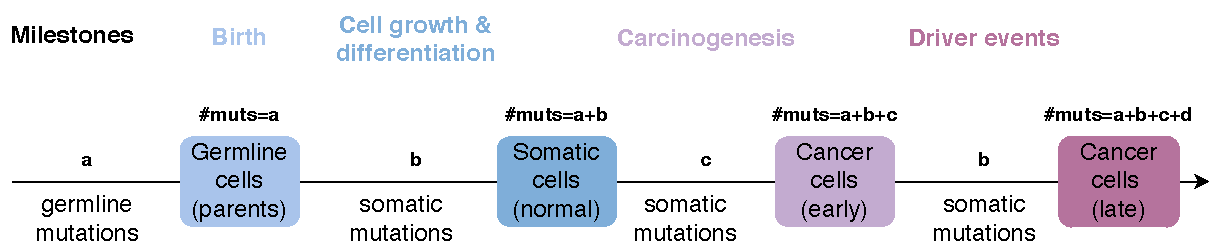
\includegraphics[scale=0.78]{graphics/drivers_demo.pdf}
    \caption{\textbf{Timeline of a carcinogenesis process.} Mutations are generally retained in the genome after each stage of carcinogenesis, even though carcinogenesis and driver events could change the phenotype of the cells. Together, all mutations available in a cancer cell make up it mutation profile. For the purpose of this project, only somatic mutations are considered because germline mutations are not the product of the environment of the differentiated cells in which cancer develop.}
    \label{fig:drivers_demo}
\end{figure}
